
\section{Introduction}
\label{sec:intro}

The credit card fraud detection problem stands as a crucial pillar in large financial system. It is important that credit card companies are able to recognize fraudulent credit card transactions so that customers are not charged for items that they did not purchase. Our main focus is to develop a preditor to recognize the fraudness using the related financial data.

A dataset has been collected containing European cardholders in September 2013 to enable the development and evaluation of effective credit card fraud detection models. The purpose of this dataset is to aid credit card companies in recognizing fraudulent transactions to ensure that customers are not charged erroneously for purchases they did not make.

The dataset consists solely of numerical variables resulting from a Principal Component Analysis (PCA) transformation. Aside from \textit{Time} and \textit{Amount}, which were not transformed using PCA, features V1 through V28 represent the principal components obtained from the PCA analysis. \textit{Time} represents the elapsed time (in seconds) between each transaction and the first transaction in the dataset, while \textit{Amount} represents the amount of the transaction. The feature \textit{Class} is the response variable and takes a value of 1 if the transaction is identified as fraudulent, and 0 otherwise.

The dataset includes transactions that occurred over a period of two days, where there were 492 instances of fraud out of 284,807 total transactions. It is worth noting that the dataset is highly unbalanced, as the positive class, i.e. fraud, accounts for only 0.172\% of all transactions, which is shown in Figure \ref{fig:ClassDistribution} and Figure \ref{fig:TransactionAmount}.

Given the highly unbalanced nature of the dataset, with a small proportion of fraud cases, the challenge lies in accurately identifying instances of fraud while minimizing false positives. This imbalance poses a significant problem for machine learning algorithms to learn effectively.


Addressing this issue requires the development of advanced machine learning techniques, such as anomaly detection, class imbalance handling, or algorithmic adjustments for cost-sensitive learning. These approaches aim to improve the detection accuracy of fraudulent credit card transactions, ultimately benefiting both credit card companies and their customers by reducing financial losses and ensuring trust and security in financial transactions.

The rest of this paper is organized as follows: Some anomaly detection methods will be applied in Section \ref{sec:outliers}. In Section \ref{sec:imbalance}, we will focus on the issue of data imbalance, for which some methods will be applied. In Section \ref{sec:machine}, we develop some machine learning methods to solve the problem, and show some results afterwards. Some conclusion remarks will be made in Section \ref{sec:conc}.


\begin{figure}[htbp]
	\centering
	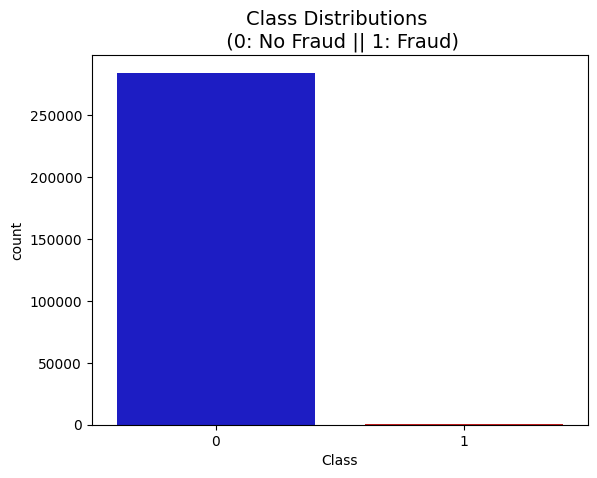
\includegraphics[width=0.7\linewidth]{../output7}
	\caption[Class Distribution]{Class Distribution}
	\label{fig:ClassDistribution}
\end{figure}

\begin{figure}[htbp]
	\centering
	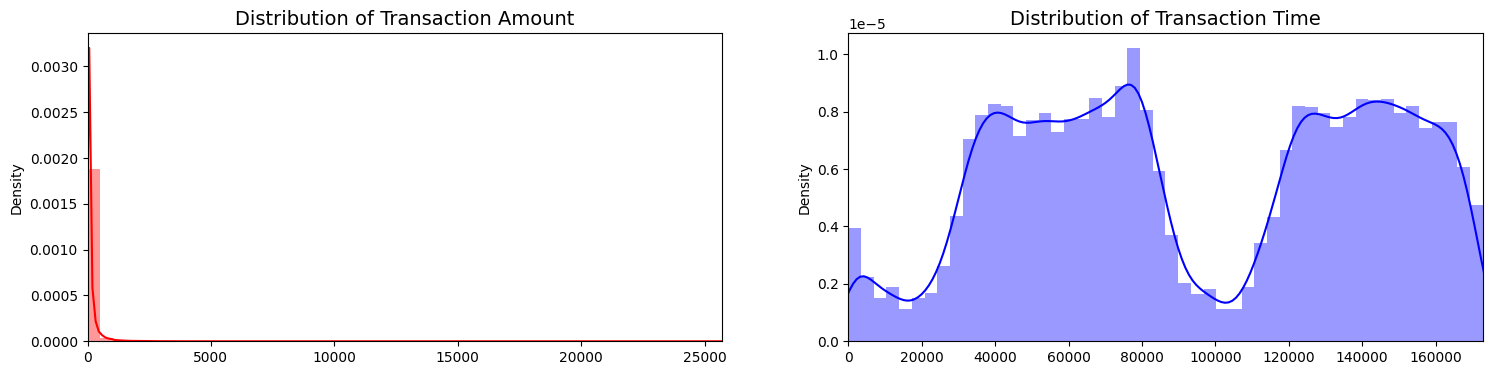
\includegraphics[width=0.7\linewidth]{../output8}
	\caption[Transaction Amount and Time Distribution ]{Transaction Amount and Time Distribution}
	\label{fig:TransactionAmount}
\end{figure}











\section{Outliers: Anomaly Detection}
\label{sec:outliers}
\subsection{Introduction to Anomaly Detection}

Anomaly detection is a method of identifying observations or data that are considered unusual or abnormal compared to the rest of the dataset. The utilization of anomaly detection provides a crucial method for identifying unusual data points that provide insight into potential errors, fraud, or malicious activity. Anomalies often translate into significant business value, such as early identification of system failure, immediate responses against fraud, or preventing security breaches. The detection of anomalies requires various techniques and algorithms, including statistical methods, machine learning, and deep learning approaches. In general, identifying anomalies in data is a complex and challenging problem, as it often requires an understanding of the dataset and context of the application.

\subsection{Methods of Anomaly Detection}

The approaches for anomaly detection span a vast range of definitions and techniques, from rule-based methods to machine learning and deep learning algorithms. Traditionally, simple statistical techniques such as clustering, regression, or classification have commonly been employed to identify anomalies in data. More recently, unsupervised machine learning methods, including k-means, isolation forest, and one-class support vector machines, have gained popularity for detecting anomalies. Deep learning techniques, such as autoencoders, convolutional neural networks, and recurrent neural networks, can also detect anomalies by learning the data's underlying representations. Additionally, there are several open-source anomaly detection frameworks available, such as PyOD and Scikit-learn, which can aid in the implementation of these methods.

\subsection{Interquartile Range Method}

\subsubsection*{Introduction}

The Interquartile Range (IQR) method is a simple and robust method for detecting outliers in a dataset. The approach is based on the distribution's interquartile range, which is a measure of the dataset's spread. This method involves calculating the first and third quartiles of the dataset and then computing the distance between them. The distance, also referred to as the IQR, is then used to determine the threshold for classifying data points as outliers.

\subsubsection*{Methodology}

The IQR method defines a data point as an outlier if it falls outside the range of the \textit{inner fence}, which is defined as
\begin{equation}
	\textrm{Inner fence} = [\textrm{Q1} - k(\textrm{IQR}), \textrm{Q3} + k(\textrm{IQR})] 
\end{equation}
where Q1 and Q3 are the first and third quartiles of the dataset, respectively, and $k$ is a scaling factor that determines the range of the inner fence. Typically, $k$ is set to $1.5$, but it can be adjusted based on the specific dataset and problem.

Data points outside the inner fence but within the \textit{outer fence} are considered mild outliers, while those above the outer fence are classified as extreme outliers. The outer fence is defined as
\begin{equation}
	\textrm{Outer fence} = [\textrm{Q1} - 3k(\textrm{IQR}), \textrm{Q3} + 3k(\textrm{IQR})]
\end{equation}

The IQR method is simple to implement and computationally efficient, making it a popular choice for detecting outliers. However, it requires that the data be roughly symmetrically distributed, and it is less effective at detecting outliers in skewed distributions.


\subsubsection*{Experiment Results}

We have to be careful as to how far do we want the threshold for removing outliers. We determine the threshold by multiplying a number, for example $1.5$, by the Interquartile Range. The higher this threshold is, the less outliers will detect, and the lower this threshold shows the opsite way.  Figure \ref{fig:vis_feature} shows the results for 3 features.

\begin{figure}[htbp]
	\centering
	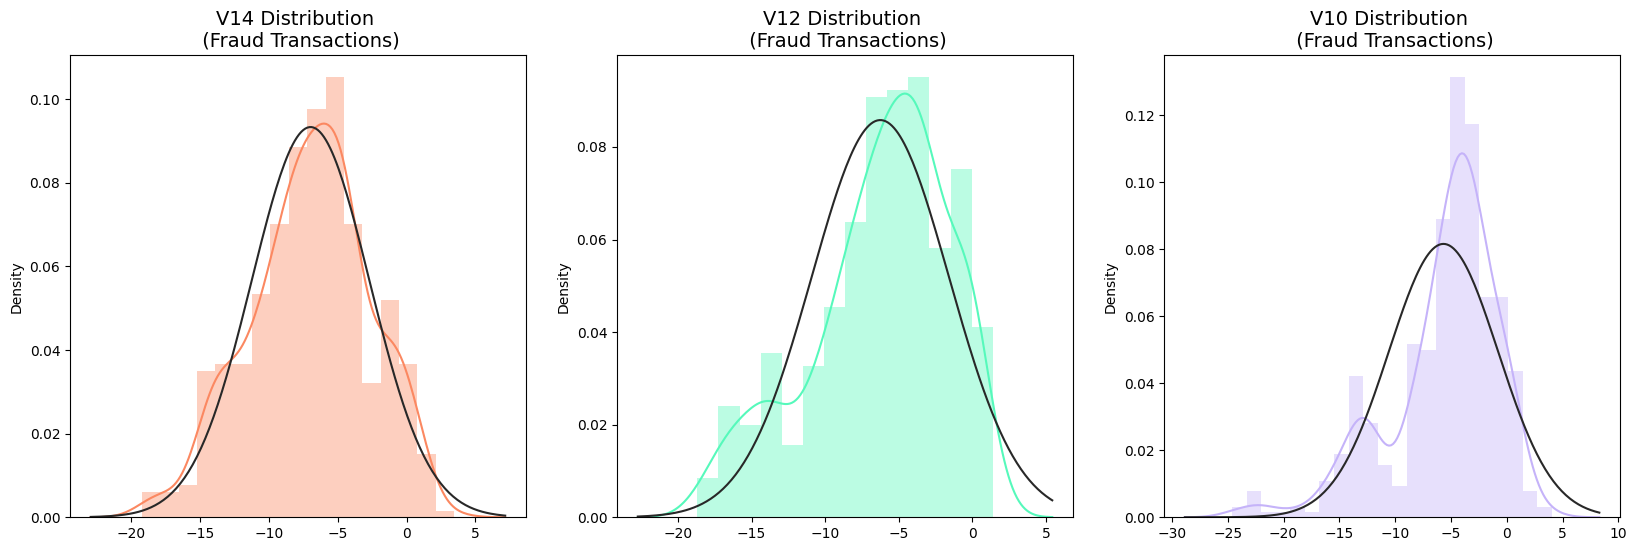
\includegraphics[width=0.7\linewidth]{../output9}
	\caption{Visualization of feature distribution}
	\label{fig:vis_feature}
\end{figure}


\subsubsection*{Tradeoff}

We want to focus more on extreme outliers rather than just outliers. We might run the risk of information loss which will cause our models to have a lower accuracy. 

 We first start by visualizing the distribution of the feature we are going to use to eliminate some of the outliers. V14 is the only feature that has a Gaussian distribution compared to features V12 and V10.
 
 After we decide which number we will use to multiply with the IQR, we will proceed in determining the upper and lower thresholds by substrating 25\% quartile threshold, i.e. the lower extreme threshold, and adding 75\% quartile threshold, i.e. the upper extreme threshold, as shown in Figure \ref{fig:vis_outliers}.

\begin{figure}[htbp]
	\centering
	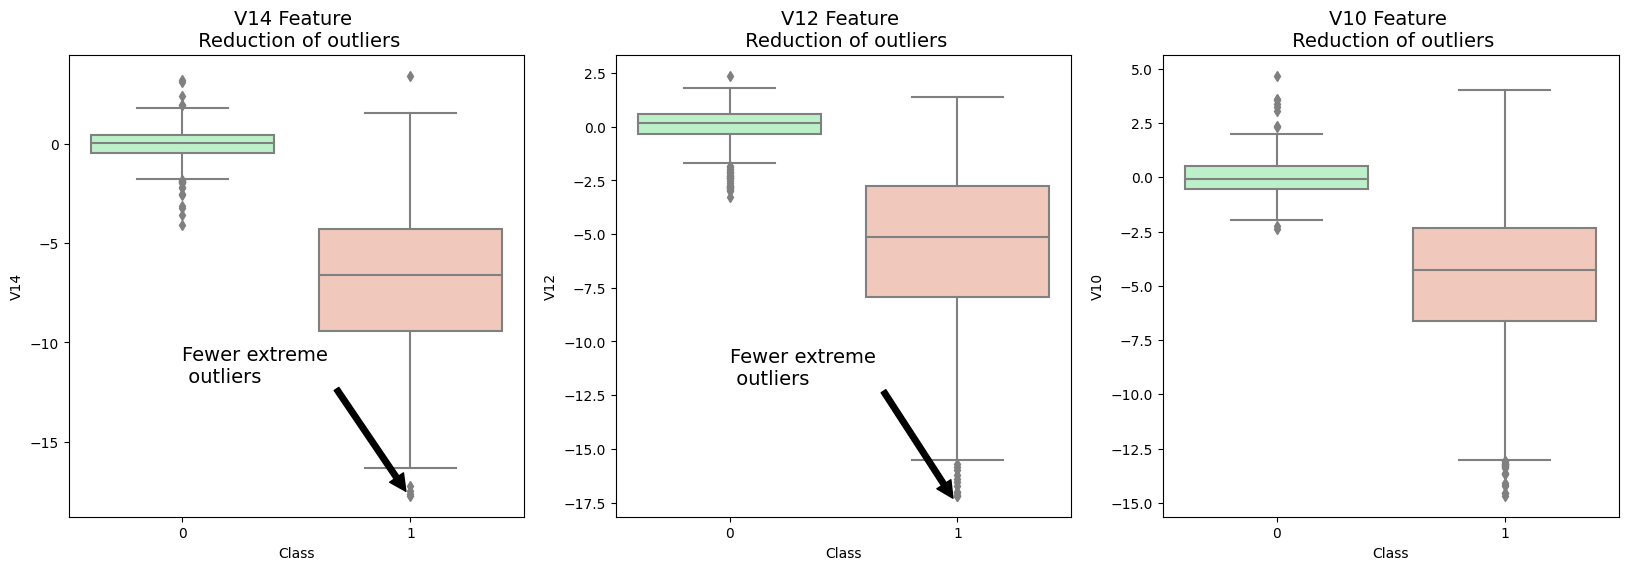
\includegraphics[width=0.7\linewidth]{../output10}
	\caption{Visualization of Outliers}
	\label{fig:vis_outliers}
\end{figure}


\section{Class Imbalance Handling Approach}
\label{sec:imbalance}


\section{Machine Learning Theory}
\label{sec:machine}

To solve this problem, we need to build a model that can detect fraudulent transactions based on the features. One possible method is to use a logistic regression model, which is a type of supervised learning algorithm that can perform binary classification. The logistic regression model estimates the probability of a transaction being fraudulent using a sigmoid function:

\subsection{Logistic Regression}

The logistic function is of the form
\[p(y=1|x) = \frac{1}{1+e^{-\theta^Tx}}\]
where $x$ is the feature vector, $\theta$ is the parameter vector and $y$ is the class label.

To train the logistic regression model, we need to find the optimal values of $\theta$ that minimize the cost function, which is defined as:

\[J(\theta) = -\frac{1}{m}\sum_{i=1}^m[y^{(i)}\log(p(y^{(i)}=1|x^{(i)}))+(1-y^{(i)})\log(1-p(y^{(i)}=1|x^{(i)}))]\]
where $m$ is the number of training examples.

We can use an optimization algorithm such as gradient descent to update $\theta$ iteratively until convergence:

\[\theta := \theta - \alpha \frac{\partial J(\theta)}{\partial \theta}\]
where $\alpha$ is the learning rate.

However, since the dataset is highly unbalanced, we may need to apply some techniques to deal with the class imbalance problem, such as oversampling, undersampling or using a weighted cost function. These techniques can help improve the performance of the model and reduce the bias towards the majority class.


\subsection{Deep Neural Network (DNN)}
In this subsection, we use DNN to develop the classifier for the credit card fraud detection problem. The predictor can be written as follows,
\[\mathbf{y} = \mathcal{F}_n\cdots\mathcal{F}_1(\mathbf{A}_1\mathbf{x}+b_1)\]
where $\mathcal{F}_k, k=1,\cdots,n$ are non-linear functions. The primary goal is to design a model that can effectively classify credit card transactions as either legitimate or fraudulent based on historical transaction data.

We set the 30 variables, including 'Time' and 'Amount', as input, and the probability predition as the output, i.e.
\[\mathrm{NN}_\theta(\mathbf{x})\approx P(\mbox{fraudulent transaction with variables } \mathbf{x}),\]
where $\mathrm{NN}_\theta$ is a sequential neural network consisting of 4 kinds of layers with parameter $\theta$:
\begin{itemize}
	\item Input layer: the input shape is determined by the number of features in the training data.
	\item Batch normalization layer: it helps stabilize training by normalizing the outputs of the previous layer, reducing internal covariate shift.
	\item Dropout layer: randomly drops a fraction of neurons during training, which helps prevent overfitting and improves generalization.
	\item Output layer: the final dense layer has 1 neuron, using the sigmoid activation function, which squashes the output between 0 and 1, making it suitable for binary classification problems.
\end{itemize}
The whole structure of the NN is shown in Table \ref{tab:NN_str}

\begin{table}[htbp]
    \centering
    \caption{The mean squared error for different regression models}
    \begin{tabularx}{\textwidth}{ p{5cm} p{6cm} L }
\toprule
    Layer&Hyperparameter&\#Parameters\\
\midrule
    Dense&256 neurons, ReLU activation&7936\\
	Batch Normalization&/&1024\\
	Dropout&dropout rate 0.3&0\\
	Dense&256 neurons, ReLU activation&65792\\
	Batch Normalization&/&1024\\
	Dropout&dropout rate 0.3&0\\
	Dense&256 neurons, ReLU activation&65792\\
	Batch Normalization&/&1024\\
	Dropout&dropout rate 0.3&0\\
	Dense&1 neuron, sigmoid activation&257\\
\bottomrule
    \end{tabularx}
    \label{tab:NN_str}
\end{table}

We use the binary cross-entropy as the loss function, that is 
\[J(\theta)=-[y\log(\mathrm{NN}_\theta(\mathbf{x}))+(1-y)\log(1-\mathrm{NN}_\theta(\mathbf{x}))],\]
where $y$ denotes the true value and $\mathrm{NN}_\theta(\mathbf{x})$ denotes the output of the model. and the model is compiled with the Adam optimizer using a learning rate of 1e-4.
The results for the model are shown in Figure \ref{fig:DNNr}.

\begin{figure}[htbp]
	\centering
	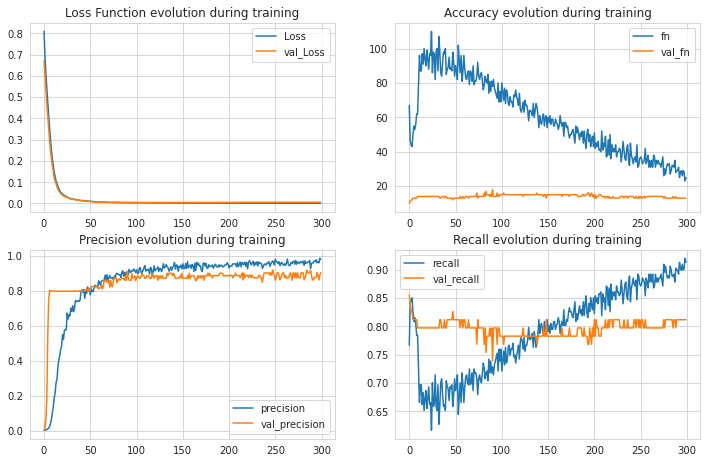
\includegraphics[width=0.7\linewidth]{DNNr.png}
	\caption{Results for DNN predictor}
	\label{fig:DNNr}
\end{figure}



\subsection{XGBoost}

In this section, we explore the implementation of an XGBoost model for credit card fraud detection. XGBoost is an advanced gradient boosting algorithm known for its high performance and effectiveness in various machine learning tasks.

The XGBoost model does not have a specific architecture like neural networks. Instead, it is an ensemble learning method that combines multiple weak structures, i.e. decision trees, to create a strong predictive model. The model employs gradient boosting to iteratively improve the performance of the decision trees, where in each iteration, the model focuses on the misclassified data points to build new trees that correct the errors of the previous ones.

We plot the AUC-ROC curve afterwards to show the validation of the model, as shown in Figure \ref{fig:XGBoost}.

\begin{figure}[htbp]
	\centering
	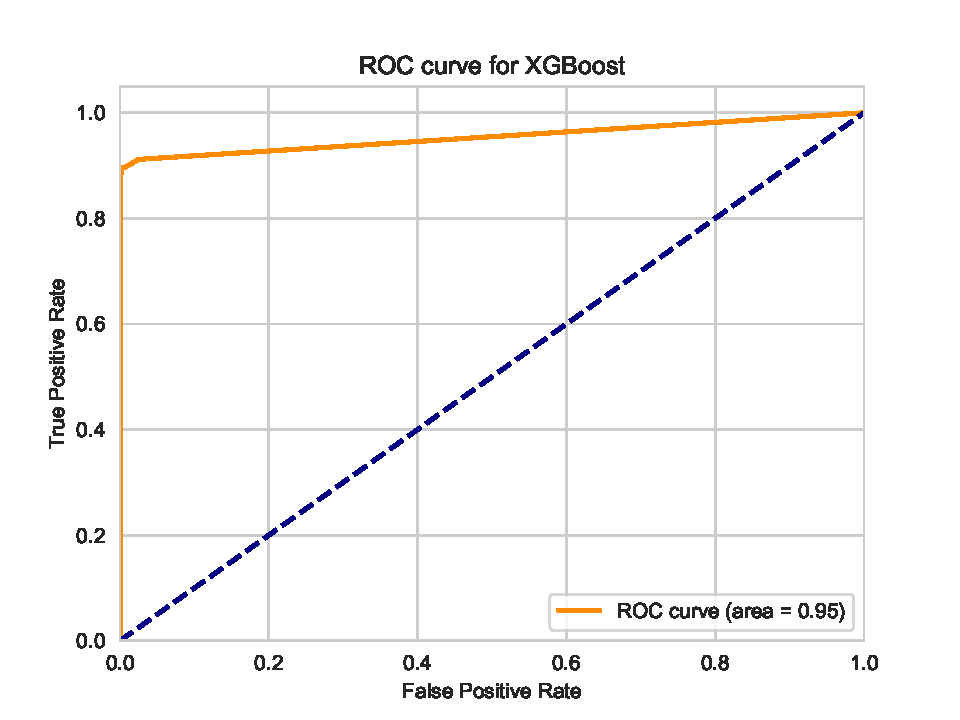
\includegraphics[width=0.7\linewidth]{xgboost.pdf}
	\caption{AUC-ROC curve for XGBoost predictor}
	\label{fig:XGBoost}
\end{figure}

\subsection{CatBoost}

Further more, we explore the implementation of the CatBoost model for credit card fraud detection. CatBoost is a high-performance gradient boosting algorithm, known for its exceptional accuracy, efficient handling of categorical features, and robustness against overfitting.

Like XGBoost, CatBoost is based on the gradient boosting framework and works by sequentially building an ensemble of weak decision trees. The central principle of CatBoost revolves around addressing the challenges posed by categorical features and optimizing the overall model performance. Compared with XGBoost, CatBoost natively handles categorical features without the need for preprocessing the lable into one-hot code. It automatically processes categorical data during training, providing a significant advantage in our detection problem. 

CatBoost introduces ordered boosting, which sorts the categorical levels, improving stability and performance compared with XGBoost. Besides, CatBoost uses symmetric trees for faster computations and also has measures to prevent overfitting. For these reasons, we hope that CatBoost can predict better in our problem, which can be also validated in Figure \ref{fig:catboost}.

\begin{figure}[htbp]
	\centering
	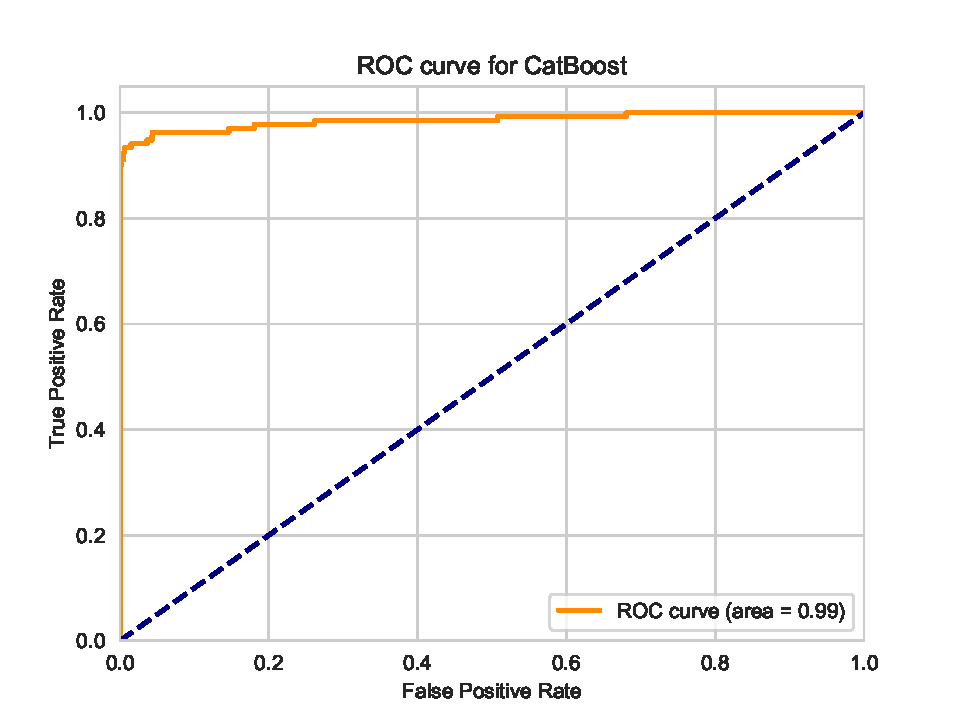
\includegraphics[width=0.7\linewidth]{catboost.pdf}
	\caption{AUC-ROC curve for CatBoost predictor}
	\label{fig:catboost}
\end{figure}



\section{Summary}
\label{sec:conc}



% R code here if necessary \begin{lstlisting}[style=cmd]
	% load('mydata.Rdata')
	% \end{lstlisting}
% \ \\

% Output of the code
% \begin{lstlisting}[style=output]
	%  this is a code in output style ...
	% \end{lstlisting}
% \ \\
% Code inline
% \lstinline[style=cmd]|this is an inline code ...|\\
% \ \\

% To add an image:
% 
\includegraphics[scale=0.5]{logoDMI.jpg} % save images in the folder img


